\documentclass[20 pts]{article}
\usepackage{xeCJK}
\usepackage{amsfonts}
\usepackage{amssymb}
\usepackage{amsmath}
\usepackage{bm}
\setCJKmainfont{SimSun}
\title{Linear Interleaver Design} 
\author{Kwame Ackah Bohulu}
\date{22-06-2017}
\begin{document}
\maketitle


\section{Introduction}
ターボ符号は二つの畳み込み符号をインタリーバで並列連結して作られている。ターボ符号の性能は有効自由距離に頼っている[3]。有効自由距離とは、入力重み2エラーイベントに関する最低距離である[2]。要素符号の周期の倍数値の入力重み2エラーイベントは低い重みをもつ符号語を出力する。なので、そのようなエラーエベントを両方の要素符号に起きることを発生することは目的である。インタリーバの働きは、2番目の要素符号器に入力する情報系列の順番を並び替えることである。一番目の要素符号器に起きる入力重み2エラーイベントを2番目の要素符号器に起きらないようなインタリーバを設計すれば、ターボ符号の有効自由距離が増加させ、性能が向上させる。


\section{長さ$d$の入力重み2エラーイベントを発生する}
入力重み2エラーイベントは、二つのビット1が入っている情報系列と言うエラーイベントである[2]。ターボ符号の場合、両方の要素符号器にある一つのエラーイベントに対応する。代表的な入力重み2エラーイベントは図1に描かれている。

\begin{figure}[h!]
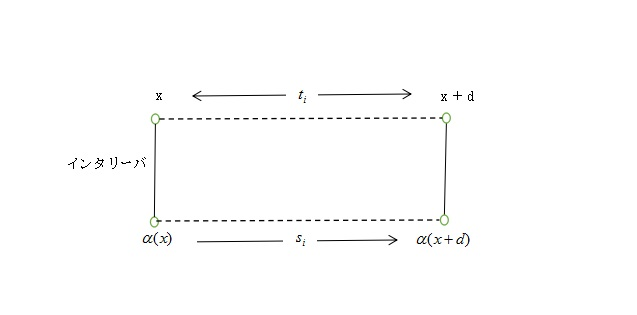
\includegraphics[width=\textwidth]{weight2error.jpg}
\caption{代表的な入力重み2エラーイベント}
\label{}
\end{figure}
一番目の要素符号で、エラーイベントは$x$から$x+d$までである。$x \in \mathbb{Z},d \in \tau \cdot \mathbb{Z} \triangleq \mathbb{C}$。  $\tau$ は要素符号器の周期である。エラーイベントの開始と終了は、整数組$(x,x+d)$で代表する。それぞれ位置をインタリーバで位置$\alpha(x)$と$\alpha(x+d)$に並び替えて、その距離は $(\alpha(x+d),\alpha(d)) \triangleq \alpha(x+d) - \alpha(d) $である。$d \in \mathbb{C}$なので、$a\tau$に書き換えられる。$a$は小さい整数値である。
 

両方の要素符号に周期の小さい倍数値の長さを持つ入力重み2(種類1)エラーイベントがある場合、ターボ符号のビット誤り率(BER)性能に与える影響をわかるようになりたいである。最尤復号とAWGNチャネルの場合、畳み込み符号のビット誤り率性能は組合結合技術で上界できる[2]。


\begin{equation}
P_b \leq \sum_{i=1}^{2^N} \frac{w_i}{N}Q\Bigg( \sqrt{d_i\frac{2RE_b}{N_o}}\Bigg)
\end{equation}
 $w_i$ と $d_i$は$i$番目の符号語の組織ビットの重みと合計ハミング重みである。ターボ符号は畳み込み符号から作られているので、(1)でターボ符号のビット誤り率性能の上界が計算できる。



ターボ符号に関する種類1エラーイベントの合計出力重みは以下の式で計算できる[1]

\begin{equation}
w_{(t_i,s_i)}=6+\Bigg( \frac{\sum \left|t_i\right|}{\tau} + \frac{\sum \left|s_i\right|}{\tau} \Bigg)w_o
\end{equation}

$t_i$と$s_i$はそれぞれの要素符号に起きる種類1エラーイベントの長さで、$w_o$は$1+D^\tau$の形を持つ入力系列の場合、一番目の要素符号の出力の重みである。$t_i$と$s_i$は$\tau$の倍数値なので、$a\tau$に書き換えることができ、$a =\{1,2,3\}$

$t_i$と$s_i$を調整するこで、同じ合計ハミング重みを持つ符号語が集められ、符号語あたりの平均組織ビット重みは以下のように定義する[1]。 

$$ w_d=\frac{W_d}{N_d}$$

$W_d$は重み$d$を持つ符号語の合計組織ビットの重みで、 $N_d$は重み$d$を持つ符号語の数である。。それで、(1)を書き換えると、式3が出る。


\begin{equation}
P_b \lessapprox \sum_{d=d_{(a=1)}}^{d_{(a=4)}} \frac{N_dw_d}{N}Q\Bigg( \sqrt{d\frac{2RE_b}{N_o}}\Bigg)
\end{equation}
3種類の要素符号を使用するターボ符号のビット誤り率の図が図2に描かれている。
\begin{figure}[h!]
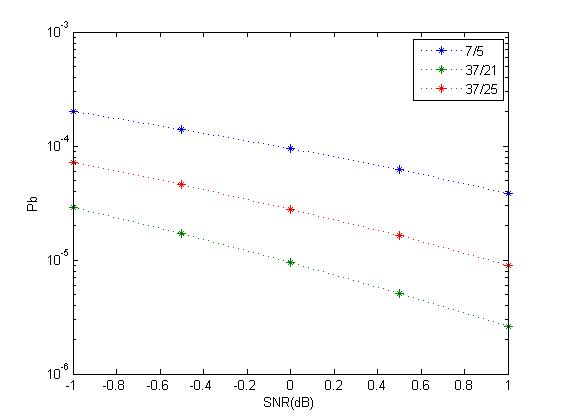
\includegraphics[width=\textwidth]{berValues.jpg}
\caption{3種類の要素符号を使用するターボ符号のビット誤り率、N=1024}
\label{}
\end{figure}
以下の状況を満足するインタリーバを設計したいです。
 $$(\alpha(x+d),\alpha(d)) \notin \mathbb{C} \triangleq \mathbb{E}(\alpha(x+d),\alpha(d)) \\\\\ \forall x \in \mathbb{Z} , d \in \mathbb{C}$$ 


\subsection{線形インタリーバの設計}
提案されたインタリーバのマッピング関数は式4で定義されている。
\begin{equation}
\alpha(x)_{\mathfrak{L}_N}=x(\tau^2 - z\tau + 1) \mod N
\end{equation}
$N = 2^n, n\in \mathbb{R}$ インタリーバの大きさで、$z$は範囲1 から $\sqrt{2N}$までの最大奇数値である。

$n$の値が3から10まで、$\tau$の値が2から7まで、そして$a$の値がは1から3までの場合、$(\alpha(x+d),\alpha(d))$の値が表1から3に書かれている。
\begin{table}[h!]
\centering
\begin{tabular}{ |p{0.7cm}|p{0.7cm}|p{0.7cm}|p{0.7cm}|p{0.7cm}|p{0.7cm}|p{0.7cm} |p{0.7cm}||p{0.7cm} |}
 \hline
 \multicolumn{8}{|c|}{$N=2^n$, $(\alpha(x+d),\alpha(x))$} \\
 \hline
n=3&n=4&n=5&n=6&n=7&n=8&n=9&n=10&$\tau$\\
 \hline
  6  &   6  &   6  &  30 &   70 &  174 &  390 &854&2\\
  1 &    1 &   13&    59 &    5  &  79 &  245 &649&3\\
 4  &   4 &   20 &   20 &   52 &  212 &   52 & 372&4\\
5  &   5 &    1 &   47 &   89  &  67 &  329 & 29&5\\
 2  &  10  &  26  &  18 &  122  & 162 &   58 &650&6\\
1   &  9  &   5   &  3 &   29 &  247 &  269 &193&7\\

 \hline
\end{tabular}
\caption{$(\alpha(x+d),\alpha(x))$の値, a=1}
\label{table:1}
\end{table}


\begin{table}[h!]
\centering
\begin{tabular}{ |p{0.7cm}|p{0.7cm}|p{0.7cm}|p{0.7cm}|p{0.7cm}|p{0.7cm}|p{0.7cm} |p{0.7cm}||p{0.7cm} |}
 \hline
 \multicolumn{8}{|c|}{$N=2^n$, $(\alpha(x+d),\alpha(x))$} \\
 \hline
n=3&n=4&n=5&n=6&n=7&n=8&n=9&n=10&$\tau$\\
 \hline
   
   4   & 12  &  12  &  60  &  12  &  92 &  268 &  684  &   2\\
   2   &  2   & 26   & 54   & 10  & 158 &  490 &  274  &   3\\
   0   &  8  &   8  &  40 &  104  & 168 &  104 &  744  &   4\\
   2   & 10 &    2  &  30  &  50  & 134  & 146  &  58  &   5\\
  4    & 4   & 20  &  36  & 116  &  68 &  116  & 276  &   6\\
  2    & 2   & 10   &  6  &  58  & 238  &  26  & 386   &  7\\

 \hline
\end{tabular}
\caption{$(\alpha(x+d),\alpha(x))$の値, a=2}
\label{table:2}
\end{table}

\begin{table}[h!]
\centering
\begin{tabular}{ |p{0.7cm}|p{0.7cm}|p{0.7cm}|p{0.7cm}|p{0.7cm}|p{0.7cm}|p{0.7cm} |p{0.7cm}||p{0.7cm} |}
 \hline
 \multicolumn{8}{|c|}{$N=2^n$, $(\alpha(x+d),\alpha(x))$} \\
 \hline
n=3&n=4&n=5&n=6&n=7&n=8&n=9&n=10&$\tau$\\
 \hline
  
   2  &   2  &  18   & 26   & 82  &  10 &  146 &  514  &   2\\
   3 &    3  &   7  &  49  &  15 &  237 &  223 &  923 &    3\\
   4  &  12  &  28 &   60 &   28&   124 &  156 &   92  &   4\\
   7  &  15 &    3 &   13  &  11 &  201 &  475 &   87  &   5\\
   6   & 14   & 14  &  54 &  110 &  230 &  174 &  926 &    6\\
   3  &  11   & 15  &   9  &  87  & 229  & 295 &  579   &  7\\

 \hline
\end{tabular}
\caption{ $(\alpha(x+d),\alpha(x))$の値, a=3}
\label{table:3}
\end{table}
提案された線形インタリーバをターボ符号器のインタリーバとして、シミュレーションされた。シミュレーションで得られたビット誤り率性能は、図3で書かれている。

\begin{figure}[h!]
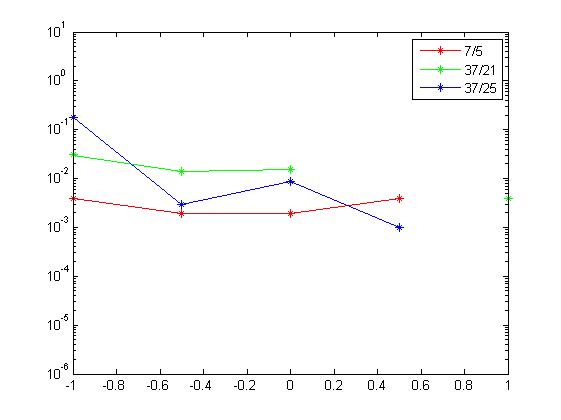
\includegraphics[width=\textwidth]{myLinearInterleaver.jpg}
\caption{シミュレーションで得られたビット誤り率性能、N=1024}
\label{}
\end{figure}

\newpage
\section{References}
\paragraph{[1]}  Oscar Y. Takeshita, Member, IEEE, and Daniel J. Costello ,''New Deterministic Interleaver Designs for Turbo Codes'',IEEE Trans. Inform. Theory, vol.  46,pp. 1988-2006,Nov. 2000\\
\paragraph{[2]}  L. C. Perez, J. Seghers, D. J. Costello, Jr., ''A distance spectrum interpretation of turbo codes'', IEEE Trans. Inform. Theory, vol. 42, pp. 1698-1709, Nov. 1996.\\
\paragraph{[3]} Jing Sun, Oscar Y. Takeshita ”Interleavers for Turbo Codes Using Permutation Polynomials over Integer Rings”, IEEE Trans. Inform. Theory, vol. 51,
pp. 101 - 119 Jan. 2005



\end{document}